\documentclass[a4paper,11pt,twoside]{report}


\title{
	\Huge{\textsf{Optical Tweezers}}
}

\author{
	\large \textsf{Marijn Venderbosch}
}

\date{\normalsize \textsf{\today}}

%essentials
\usepackage[T1]{fontenc}
\usepackage[top=1in,left=1.25in,bottom=1in,right=1in]{geometry}
\usepackage{graphicx}
\usepackage{mathtools}
\usepackage{float}
\usepackage{amsmath}
\usepackage{amssymb}
\usepackage{subcaption}
\usepackage{url}
\usepackage{hyperref}
\usepackage{chngcntr}
\usepackage{cleveref}
\usepackage{microtype}
\usepackage{subfiles}
\usepackage[toc,page]{appendix}
\usepackage{tabularx}
\usepackage{array}
\usepackage{enumitem}
\usepackage{setspace}

%braket notation00000000000000000000000000000000000000000000000000000
\DeclarePairedDelimiter\bra{\langle}{\rvert}
\DeclarePairedDelimiter\ket{\lvert}{\rangle}
\DeclarePairedDelimiterX\braket[2]{\langle}{\rangle}{#1 \delimsize\vert #2}

%appearance
\usepackage[labelfont={bf,sf}]{caption}
\usepackage[bf,sf]{titlesec}
\usepackage[symbol]{footmisc}
\renewcommand{\thefootnote}{\fnsymbol{footnote}}
\renewcommand{\figurename}{Fig.}
\setstretch{1.2}

%font
\usepackage[scaled=0.95]{helvet}
\usepackage{newpxtext,newpxmath}

%page header
\usepackage{fancyhdr}
\setlength{\headheight}{14pt}
\pagestyle{fancy}
\addtolength{\linewidth}{\marginparsep}
\addtolength{\linewidth}{\marginparwidth}
\renewcommand{\chaptermark}[1]{\markboth{\thechapter\ #1}{}}
\renewcommand{\sectionmark}[1]{\markright{\thesection\ #1}}
\fancyhf{}
\cfoot{\textsf{\thepage}}
\fancyhead[LE]{\textsf{\textsl{{\rightmark}}}}
\fancyhead[RO]{\textsf{\textsl{{\leftmark}}}}
\fancypagestyle{plain}{%
	\fancyhead{} % get rid of headers
	\renewcommand{\headrulewidth}{0pt} % and the line
}

%bibliography
\usepackage[backend=bibtex,sorting=none,url=false,isbn=false]{biblatex}
\addbibresource{jabref/jabreflibrary.bib}


%add scripts
\usepackage{listings}
\usepackage{color}
\definecolor{dkgreen}{rgb}{0,0.6,0}
\definecolor{gray}{rgb}{0.5,0.5,0.5}
\definecolor{mauve}{rgb}{0.58,0,0.82}
\lstset{frame=tb,
	language=Matlab,
	aboveskip=3mm,
	belowskip=3mm,
	showstringspaces=false,
	columns=flexible,
	basicstyle={\small\ttfamily},
	numbers=none,
	numberstyle=\tiny\color{gray},
	keywordstyle=\color{blue},
	commentstyle=\color{dkgreen},
	stringstyle=\color{mauve},
	breaklines=true,
	breakatwhitespace=true,
	tabsize=3
}

%Table of contents
\setcounter{tocdepth}{4}


\begin{document}
	
	
	%UNCOMMENT THE INPUT COMMAND BELOW TO ADD TITLEPAGE AND ABSTRACT
	
	%	%%%titlepage
\pagenumbering{roman}

\begin{titlepage}
	\begin{centering}
		\vspace*{2cm}
		
		\textsf{\LARGE \textbf{Titel}}
		
		\vspace{2.5cm}
		
		\textsf{\large Marijn Venderbosch}
		
		\vspace{2cm}
		
		\textsf{\large Supervisors:}
		
		\vspace{0.5cm}
		
		\textsf{\large dr. E.J. Vredenbregt\\
			dr. S. Kokkelmans}
		
		\vfill
		
		\begin{figure}[h]
			\centering
			
\includegraphics[width=6cm]{figures/logo.png}
		\end{figure}
		
		\textsf{Coherence \& Quantum Technology group (CQT)}
		
		\vspace{0.4cm}		
		
		\textsf{\today}
		
		\vspace{1cm}
		
		
	\end{centering}
\end{titlepage}
\newpage



	%\newgeometry{top=2cm,left=4cm,right=4cm,bottom=2cm}
\begin{abstract}
	
typ hier abstract

\end{abstract}
\restoregeometry


\newpage


	
	
	
	\tableofcontents
	\newpage
	
	
	\pagenumbering{arabic}
	
	
	
	\chapter{Introduction}\label{introduction}\section{Quantum Computing test}

Quantum computers have been attracting interest in the last couple of decades based on their potential ability to exponentially outperform classical computers. This was first suggested by Richard Feynman in 1982, where he argued that a classical computer modeling a quantum mechanical system would be hindered by an exponential slowdown \cite{Feynman1982}. This is relevant because a large part of computational work in the world is dedicated to solving quantum mechanical problems, e.g. for the engineering of novel materials in nanotechnology and predicting the 3D-structure of proteins for drug discovery \cite{Robert2021}.

As for how this speedup is achieved, so first hint for this resides in the exponentially growing state space of a quantum memory register: a register consisting of qubits (2-level quantum systems). An arbitrary qubit can be denoted as the superposition of two basis states, here denoted as $\ket{0}$ and $\ket{1}$: $\ket{\psi} = \alpha \ket{0} + e^{i \phi} \beta \ket{1}$, where $\phi$ is an arbitrary phase factor. The norm of  $\ket{\psi}$ is assumed normalized, a convenient way of representation is thus to choose the vector to lie on the unit sphere, absorbing the one unit of freedom of the coefficients in an angle $\theta$, letting $\phi$ keep track of the phase factor: NEGEER DIT DIT IS EEN TESTJE OK

\begin{equation}\label{eq:qubit}
	\ket{\psi} =
	\cos{\frac{\theta}{2}} \ket{0} + e^{i \phi} \sin{\frac{\theta}{2}} \ket{1}.
\end{equation}

This is called the Bloch sphere representation \cite{Nielsen2011}, shown in \cref{fig:BlochSphere}. The interesting thing about quantum computer however, arises when using multiple qubits. It can be shown that for a configuration of entangled qubits, the dimension of their tensor product scales exponentially in dimension as $2^N$ where $N$ is the number of qubits \cite{Nielsen2011,Henriet2020}. Because of this powerful result, a register consisting of 300 qubits can contain as much information $2^{300} \approx 10^{80}$ classical bits, which is roughly the number of elementary particles in the observable universe.

People have come up with algorithms that can make use of this exponentially growing Hilbert space, using the concept of quantum parallelism \cite{Nielsen2011}. For example, in Grover's algorithm, randomly searching in an unordered database they can offer a quadratic 'quantum speedup' \cite{Grover1996}. Another well-known one is Shor's algorithm for deciphering RSA encryption \cite{Shor1994}, which has been shown \cite{Vandersypen2001} to run in sub-exponential time instead of exponential time.

\begin{figure}
	\centering
	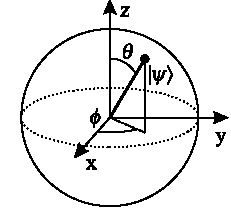
\includegraphics[width=5cm]{figures/BlochSphereCropped.pdf}
	\caption{The Bloch sphere representation. The wave function of a pure state $\ket{\psi}$ can be represented as a point on unit sphere with coordinates $\theta$ and $\phi$ \cite{Jones2012}.}
	\label{fig:BlochSphere}
\end{figure}

\subsection{The NISQ Era}

Effectively utilizing the advantages of quantum computing is not trivial. For example, the superposition state in \cref{eq:qubit} cannot be measured, so the final result of the computation should be some combination of basis states that can be measured. Additionally, there is the main enemy of quantum information: decoherence; meaning qubits lose their quantum properties because of interactions with the outside world. So to make an effective quantum computing system, the qubits have to be shielded from the outside. Decoherence that inevitably is always present can be fixed by quantum error correction (QEC) techniques \cite{Ladd2010,Preskill2018}, but requires a significant overhead in the number of qubits needed \cite{Gottesman2009,Preskill2018} and is unachievable in the near future. It is unclear whether quantum computers will ever universally outperform classical computers.

Until this fault-tolerant quantum computing is achieved, quantum computing is called to be in the \textit{noisy intermediate scale quantum} (NISQ) era \cite{Preskill2018}. Noisy in the sense that there is imperfect control over the qubits, meaning that after a finite number of gate operations, the signal to noise ratio would become too high and the qubits are not error-corrected. Still, even in the order of 50 qubits or so, NISQ machines can already potentially outperform its classical equivalent as recently demonstrated \cite{Arute2019}, achieving so-called quantum supremacy \cite{Preskill2012}.

\subsection{The Best of Both Worlds}

In the NISQ era, algorithms are needed that are not too sensitive to fidelity errors. Additionally, it should be able to run with low decoherence times \cite{McClean2016}. One such candidate is the quantum variational eigensolver (VQE), originally proposed by Perruzo and McClean \cite{Peruzzo2014}. VQE is said to work well in the NISQ era because it is effective at leveraging the strength of a quantum system as effectively as possible while keeping error propagation minimized \cite{McClean2016}. In its core, VQE essentially tries to find approximately the ground state of a quantum mechanical system according to the variational principle in quantum mechanics \cite{Griffiths2004}, which states that the expectation value of a given Hamiltonian $H$ will always be an upper bound for the ground state energy $E_g$:

\begin{equation}
	\left\langle H \right\rangle = \left\langle \psi | H | \psi \right\rangle \geq E_g.
\end{equation}

However, entangled trial states $\ket{\psi}$ cannot be efficiently initialized into a classical computer. Therefore, this state is prepared in the quantum computing unit (QPU), a dedicated hardware component working in tandem with a classical central processing unit (CPU). Therefore, this is called a hybrid quantum computer, making use of the best of both worlds. The algorithm makes use of a feedback loop continuously feeding results from the CPU to the QPU and the other way around. This process is repeated in iterations.

Here, a short summary of how VQE works will be provided, but the reader is referred to the supplied sources for a more thorough coverage. The algorithm starts by feeding an ansatz for the wave function into the QPU, shown in \cref{fig:VQE}, where it is prepared. Subsequently, the expectation value $\left\langle H\right\rangle$ of the ansatz is measured by adding individual contributions. Next, the CPU uses a classical non-linear optimizer to find a new iteration for the wave function to feed back into the QPU. This procedure is reiterated until convergence \cite{McClean2016,Peruzzo2014,Keijzer2021}.

\begin{figure}
	\centering
	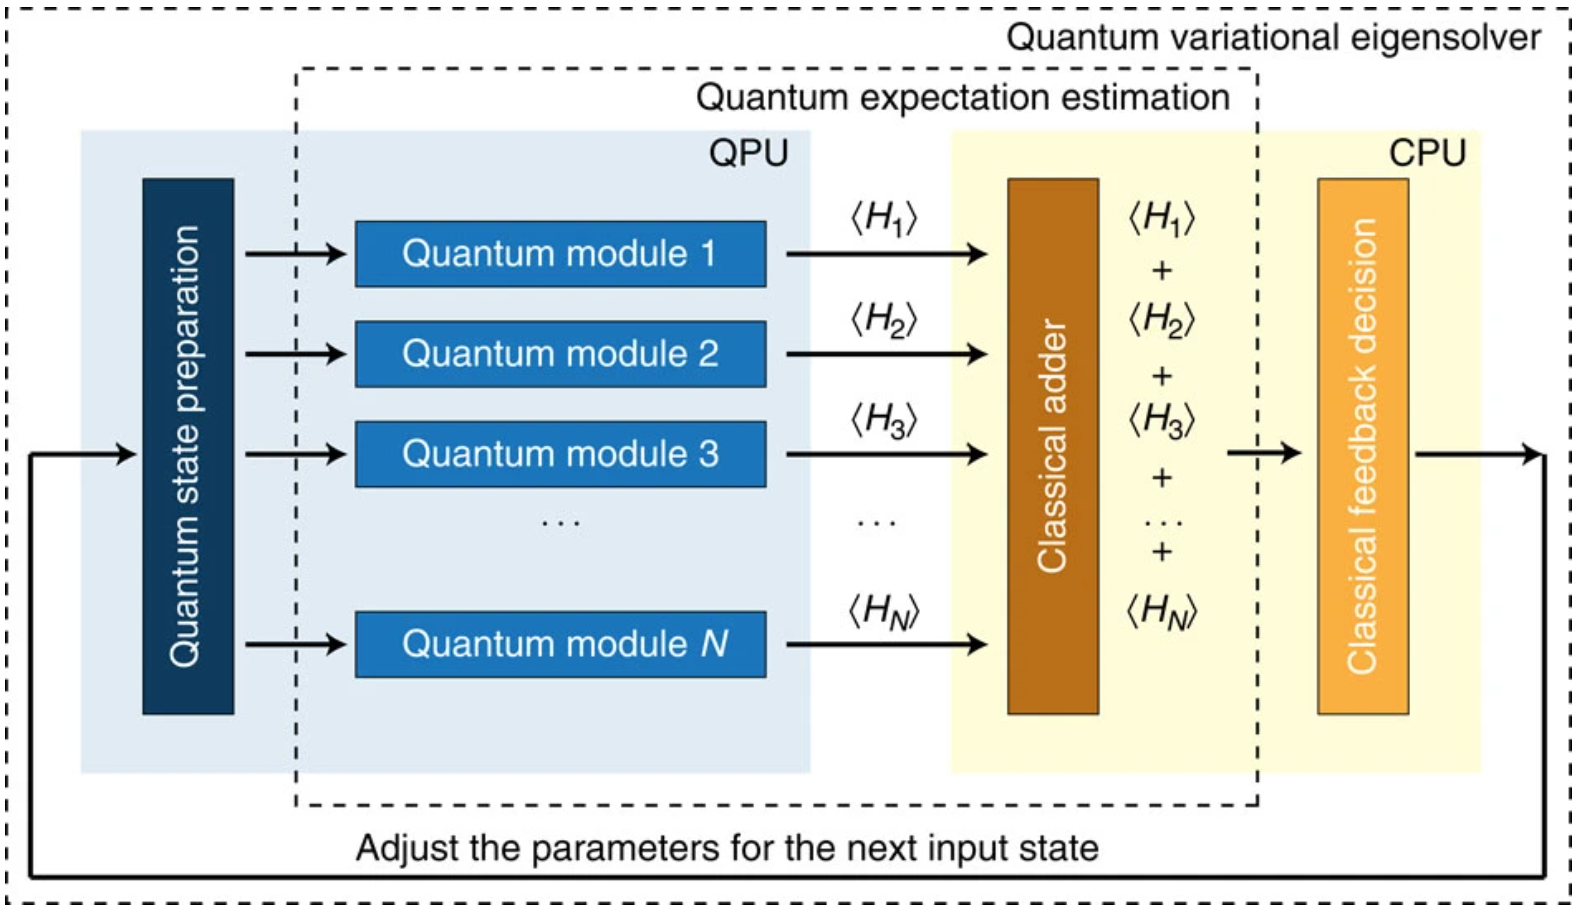
\includegraphics[width=10.5cm]{figures/vqe.png}
	\caption{The quantum variational eigensolver visualized. The algorithm is iterative, starting from an ansatz for the wave function it is prepared and the expectation value of its Hamiltonian is computed. This is fed to the CPU, which uses a non-linear optimization to find a new ansatz that will decrease the expectation value of $H$. This is repeated until convergence. \cite{Peruzzo2014}}
	\label{fig:VQE}
\end{figure}


\section{Physical Implementation}

DiVincenzo came up with a list of criteria a physical implementation of a quantum system should adhere to \cite{DiVincenzo2000}. The implementation is challenging because some criteria appear to be conflicting: state preparation, long coherence times, universal gate operation and readout. Based on the criteria, people have come up with numerous quantum systems \cite{Ladd2010}. Examples include: infrared photons \cite{Matthews2009}, trapped neutral atoms \cite{Treutlein2004}, trapped ions \cite{Benhelm2008}, electron spins \cite{Press2008} and superconducting circuits \cite{Arute2019,DiCarlo2009}.

This work will be on trapped and laser cooled neutral atoms excited to Rydberg states in an array of optical tweezers. This is a promising solution because multi-qubit gates are natively realized and the technology is scalable to a couple thousand qubits \cite{Henriet2020}.

\subsection{Trapped Neutral Atoms}

Neutral atoms trapped into an array of optical tweezers are a promising candidate to implement a quantum computer. The qubit states are encoded into the hyperfine levels of the items, which provide long decoherence times \cite{Henriet2020}. Promising atoms are in the alkali group like Rb, Cs and Sr. The main tool to interact with the atoms is laser light. Atoms are loaded in a 3D magneto optical trap (MOT) in a vacuum system, which creates in one dimension a force of the form: $F \sim -\alpha x - \beta v$, where $x$ is the position and $v$ the velocity along that dimension \cite{Metcalf1999}. Thus the atoms are trapped and cooled. The MOT is a starting point for other trapping and cooling techniques.

Subsequently, a second laser system creates an array of \cite{Schlosser2001,Bergamini2004} optical dipole traps, by shining trapping laser light onto a spatial light modulator (SLM), a device capable of creating an intensity pattern in the far field by locally adjusting the phase difference the reflected light picks up \cite{Bijnen2015}.

\subsubsection*{Optical Dipole Trap}

The first optical dipole trap was realized by Chu \textit{et al.} \cite{Chu1986}. The electric field of the laser light will cause an AC stark shift, resulting in a dipole potential scaling as \cite{Metcalf1999,Muldoon2012}

\begin{equation}
	U_{dip} \sim \frac{\hbar \Omega^2}{4\delta},
\end{equation}

where $\hbar$ is the usual reduced Planck's constant, $\Omega$ is the Rabi frequency and $\delta$ the detuning of the laser defined as the difference between the laser frequency transition frequencies: $\delta = \omega - \omega_0$. For $\delta<0$ ('red'-detuned) laser light, the dipole potential is negative and the atoms are trapped.

The dipole traps are extremely narrow: their volume is in $\mathcal{O}(\mu \text{m}^3)$. As a result, dynamics are dominated by two-body losses and the loading is sub-Poissonian \cite{Schlosser2002,Browaeys2016}. Consequently, the trap is either empty or occupied by a single atom, both with 50\% probability. To see which traps are occupied, fluorescent light is from the atoms collected onto a CCD camera. To create a full register, traps can be moved by another laser controlled by an acoustic optical deflector. An algorithm will compute for a given register filling configuration the smallest amount of steps needed to create a fully occupied array \cite{Barredo2016}, after which computation can start.

To realize computational gates, the atoms need to interact with each other. This is realized by exciting them to Rydberg states. By tuning the interactions between the qubits, computational gates can be realized.


\subsection{Rydberg States}

The individual atoms in the tweezers array are separated by a distance in the order of a couple $\mu$m, which is extremely large compared to the atom size. As a result, two-body interactions will be practically non-existent, and the atoms are not entangled which is necessary for quantum gate realization.

As a possible solution for this, the outer electron of the (alkali) atom can be excited to a very high principal quantum number $n$ in $\mathcal{O}(10^2)$, the so-called Rydberg state. Rydberg states have exaggerated interaction strengths. For example, their polarizability scales as $n^7$. The highest order scaling occurs for the der Waals coefficient, scaling as $n^{11}/R^6$ where $R$ is the distance between two atoms \cite{Gallagher1994}. Because of this, interactions are possible even for large $R$.

Quantum logic can be achieved using the Rydberg blockade effect, originally proposed by Jaksch \textit{et al.} \cite{Jaksch2000}. Consider the situation for an individual qubit: situation a) in \cref{fig:RydbergBlockade}. The Rydberg level $\ket{r}$ is coupled to the ground state by $\ket{g}$ by the driving frequency $\Omega$. Now when we consider a two-atom system in b) (\cref{fig:RydbergBlockade}), as a result of the mutual Van der Waals interaction, the energy levels are shifted and the double Rydberg state $\ket{rr}$ is no longer resonant, it is blocked.

In short, when you apply a driving pulse $\Omega$, atom B will only transition $\ket{g} \rightarrow \ket{r}$ if atom A is not already in $\ket{g}$. This logic naturally translates to a CNOT gate and together with the ability to manipulate individual qubit states constitutes a universal set of quantum gates \cite{Nielsen2011}. Similarly, the process can be repeated for $N$ sufficiently close atoms creating a maximally entangled $N$ qubit state can be created using the scheme proposed by Saffman and Mølmer \cite{Saffman2009}.

\begin{figure}
	\centering
	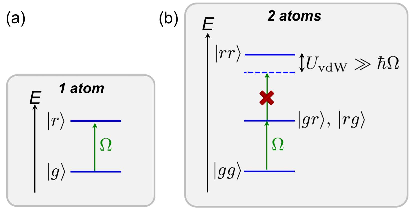
\includegraphics[width=7.5cm]{figures/RydbergBlockade.pdf}
	\caption{a) One atom: the ground $\ket{g}$ and Rydberg state $\ket{r}$ are coupled by laser frequency $\Omega$. b) Two atoms: as a result of the Van der Waals interaction between two atoms $U_{vdW}$, the states where one of the atoms is in the Rydberg state no longer couples to the double Rydberg state $\ket{rr}$. }
	\label{fig:RydbergBlockade}
\end{figure}




\section{Outline}

	%\chapter{Middle part}\label{middlepart}\input{middlepart.tex}
	%\chapter{Conclusions and Outlook}\label{conclusion}\input{conclusions.tex}
	%\chapter*{Acknowledgments}\input{acknowledgments.tex}
	
	
	
	\clearpage
	\chapter*{Bibliography}
	\addcontentsline{toc}{section}{Bibliography}%in inhoud
	
	\printbibliography[heading=none]
	
	
	
	\begin{appendices}
		
		%appendix nummering sections, equations, figures5
		\renewcommand{\thesection}{A.\arabic{section}}
		\renewcommand\thefigure{A.\arabic{figure}}
		\renewcommand\theequation{A.\arabic{equation}}
		
		\setcounter{equation}{0}
		\setcounter{figure}{0}
		
		\input{appendix.tex}
		
	\end{appendices}
	
	
	
	
\end{document} 